\chapter{Admin}
Wesentlicher Bestandteil unseres Projektes war die Administrationsumgebung. Genauer musste eine Anwendung geschaffen werden, in der Navigationsdaten hinterlegt werden k�nnen. Des Weiteren muss die Administrationsanwendung Features besitzen um Routen zu definieren und Meta-Informationen zu besonderen �rtlichkeiten festhalten zu k�nnen. Die Meta-Informationen k�nnen durch Points of Interest (PoI) Daten erweitert werden.\\
Im folgenden Abschnitt wird zun�chst die allgemeine Struktur erl�utert und anschlie�end liegt das Hauptaugenmerk auf der Benutzeroberfl�che. Eine ausf�hrliche Bedienungsanleitung der Administrationsumgebung ist im Anhang unter \nameref{Admin-Doku} beigef�gt.

\section{Allgemeine Struktur}
\subsection*{ASP.NET MVC 4}
Basis unserer Projektstruktur war das 
\textit{ASP.NET MVC Framework}\footnote{\href{http://www.asp.net/mvc}{http://www.asp.net/mvc}},
welches ein Web Application Framework ist und ein Model-View-Controller-Pattern implementiert.\\
Dies erm�glichte uns, eine Webanwendung zu entwickeln, bei der die Daten (\textit{Model}) gekapselt von der Ausgabe (\textit{View}) und dem \textit{Controller} vorliegen. Die \textit{View} pr�sentiert unsere Daten und der \textit{Controller} reagiert auf Benutzereingaben und ist sozusagen das Bindeglied oder die Schnittstelle zwischen \textit{View} und \textit{Model}.

\subsection{Model}
\subsubsection*{Account}
Diese Models wurden von MVC automatisch generiert und werden bei
der Registrierung und der An- und Abmeldung von Benutzern verwendet.

\subsubsection*{Admin}
Anwendungsspezifische Daten wie Karten, Stockwerke, Knoten, usw. werden
in selbst definierten Models gekapselt.

\subsection{View}
Die Views in unserem Projekt wurden die Bereiche Account, Admin und Home unterteilt.
\subsubsection*{Account}
Enth�lt HTML-Seiten zum Registrieren, Anmelden und Verwalten des eigenen Benutzerprofils.
\subsubsection*{Admin}
Unter diese Rubrik fallen die Webseiten, mit denen der Administrator  Stockwerke und Knoteninformationen zu einer Karte hinzuf�gen kann. Dies ist die Arbeitsoberfl�che des Administrators.
\subsubsection*{Home}
Einstiegspunkt bzw. Index unserer Webseite.

\subsection{Controller}
In unserem Projekt gibt es drei Controller.

\subsubsection*{HomeController}
Der Einstiegspunkt unserer Web-Anwendung ist der sogenannte \textit{HomeController}. Dies ist der Controller, der zum Zuge kommt, sofern die anderen beiden Controller eine Interaktion oder Controller-Aufrufe mit gewissen Parametern nicht unterst�tzen.

\subsubsection*{AccountController}
Der \textit{AccountController} verarbeitet die Ereignisse, die vom Registrierungs-, LogIn- und LogOut-Verhalten eines Benutzers ausgel�st werden. Im Fokus stehen hierbei die \textbf{HTTP GET-} und \textbf{HTTP POST-Methoden}, die von der Klasse \textit{AccountController} implementiert werden.

\subsubsection*{AdminController}
Der \textit{AdminController} reagiert auf Zustands�nderungen, die beim Anlegen, Bearbeiten und L�schen von Datenmaterial in Form von Karten oder Informationen (Meta-Informationen) ausgel�st werden.\\
Relevante Funktionen sind die Methoden zum Erstellen und L�schen von Karten und Stockwerken.
Des Weiteren werden �ber diesen Controller die Routeninformationen als Graph verarbeitet und in einer Datenbank gespeichert. Detailinformationen zu einem Knoten aus einem Graphen verarbeitet dieser Controller und speichert sie ab. Diese Detailinformationen erm�glichen besondere Orte als \textit{Points of Interest} zu kennzeichnen.

\section{Benutzeroberfl�che}
Die Admin-Oberfl�che ist �ber folgenden Link erreichbar:\\
\href{http://193.175.199.115/StudMapAdmin/}{http://193.175.199.115/StudMapAdmin/}
\begin{figure}[H]
\centering
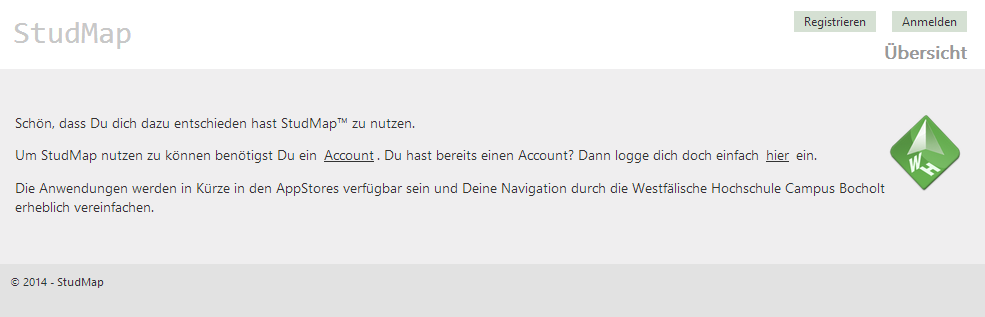
\includegraphics[width=\linewidth]{../Bilder/Admin/AdminHome}
\label{fig:AdminHome}
\end{figure}
Der Anwender hat die M�glichkeit sich anzumelden oder zu registrieren.
\subsubsection*{Registrieren}
\href{URL}{http://193.175.199.115/StudMapAdmin/Account/Register}
\begin{figure}[H]
\centering
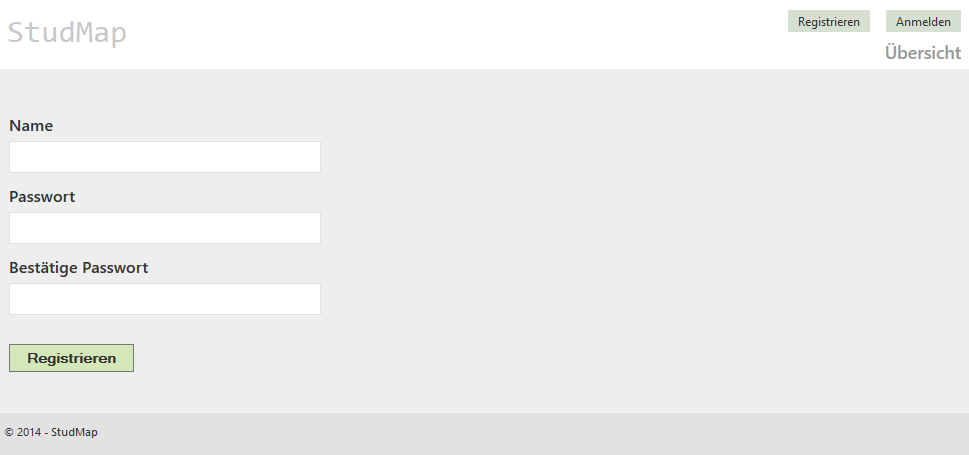
\includegraphics[width=\linewidth]{../Bilder/Admin/AdminRegistrierung}
\label{fig:AdminRegistrierung}
\end{figure}

\subsubsection*{Anmelden}
\href{http://193.175.199.115/StudMapAdmin/Account/Login}{http://193.175.199.115/StudMapAdmin/Account/Login}
\begin{figure}[H]
\centering
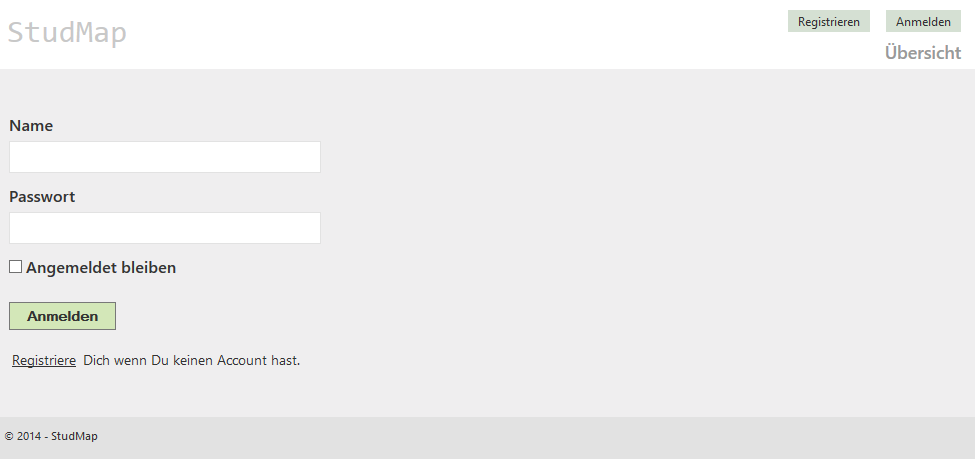
\includegraphics[width=\linewidth]{../Bilder/Admin/AdminAnmelden}
\label{fig:AdminAnmelden}
\end{figure}

\subsubsection*{Admin}
Der Einstiegspunkt zum Verwalten von Karten befindet sich unter folgendem Link: \\
\href{http://193.175.199.115/StudMapAdmin/Admin}{http://193.175.199.115/StudMapAdmin/Admin}\\
Dieser enth�lt eine Auflistung aktuell vorhandener Karten. Es  k�nnen neue Karten erstellt bzw. vorhandene entfernt werden.

\begin{figure}[H]
\centering
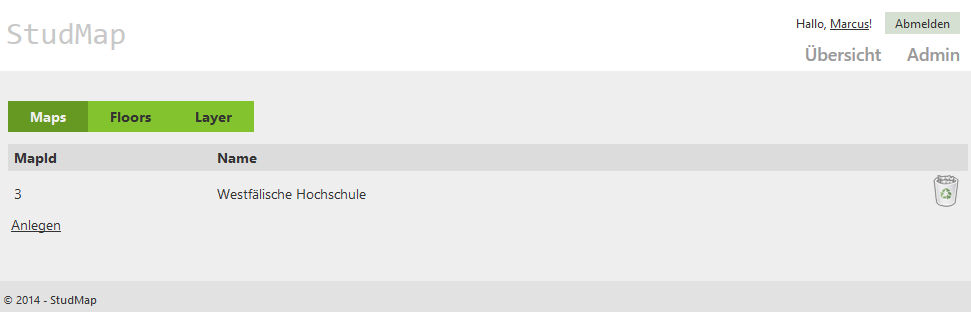
\includegraphics[width=\linewidth]{../Bilder/Admin/AdminMaps}
\label{fig:AdminMaps}
\end{figure}
Die Verwaltung der einzelnen Stockwerke zu einer Karte werden in der nachfolgenden Grafik gezeigt. Durch einen Klick auf \textit{Anlegen} kann eine neues Stockwerk mit der zugeh�rigen Kartengrundlage hinzugef�gt werden.

\begin{figure}[H]
\centering
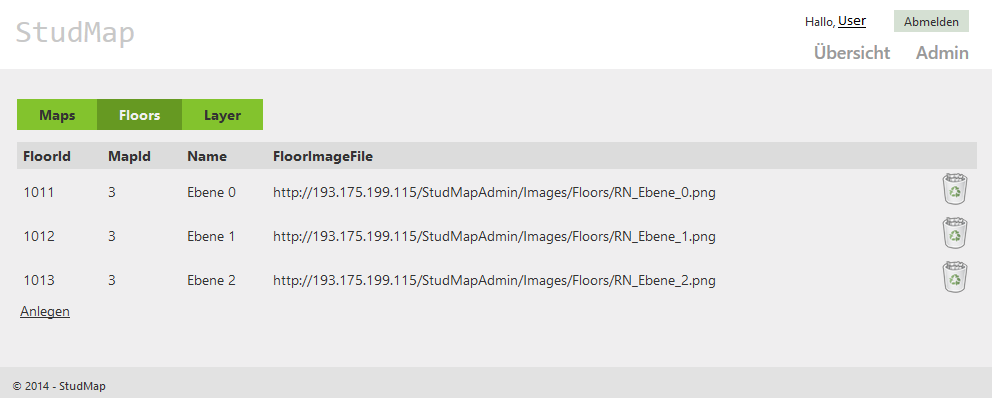
\includegraphics[width=\linewidth]{../Bilder/Admin/AdminFloors}
\label{fig:AdminFloors}
\end{figure}
Unter Layer wird die Karte und ein gegebenenfalls erstellter Graph zu genau einem Stockwerk angezeigt.
Der Administrator kann hier einen Graphen erstellen und Knoteninformationen hinterlegen. Des Weiteren besteht die M�glichkeit Knoten stockwerk�bergreifend zu verkn�pfen. Basis f�r eine ergonomische Navigation der Karte ist die JavaScript-Bibliothek \textit{D3}.

\begin{figure}[H]
\centering
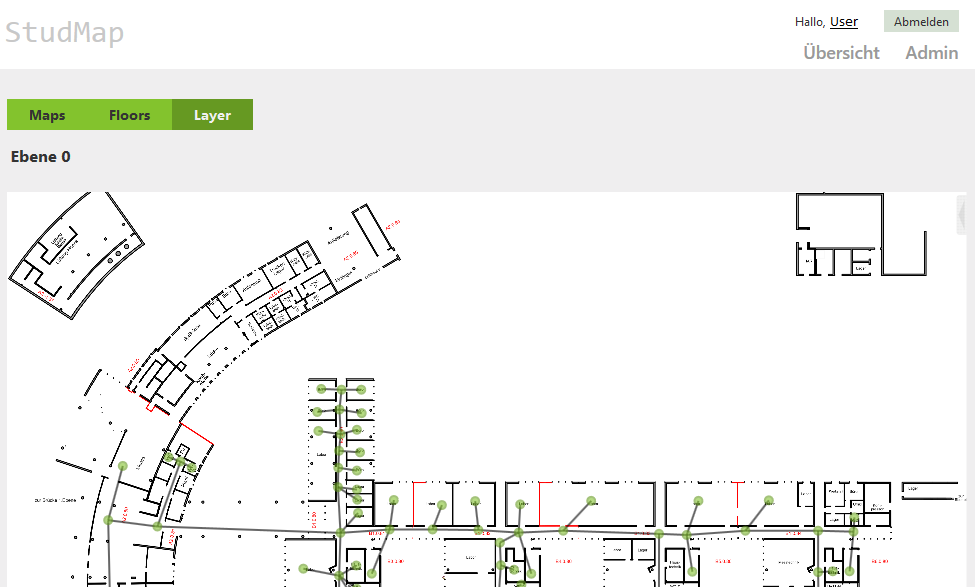
\includegraphics[width=\linewidth]{../Bilder/Admin/AdminLayer}
\label{fig:AdminLayer}
\end{figure}
\begin{figure}[H]
\centering
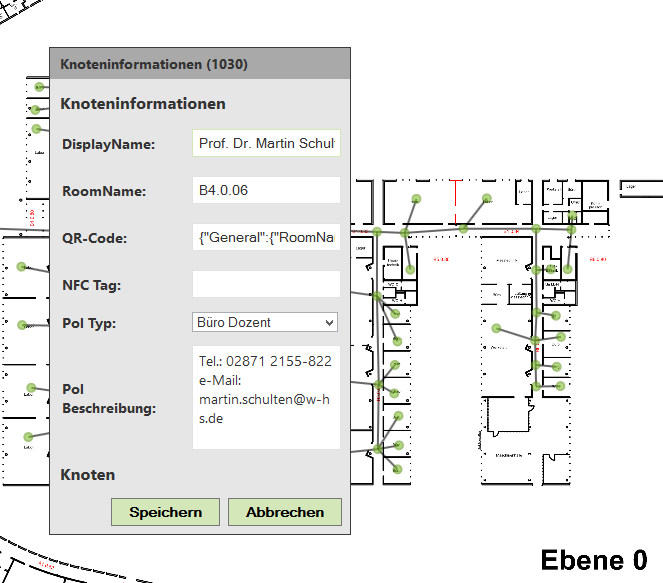
\includegraphics[width=\linewidth]{../Bilder/Admin/AdminNodeInfo}
\label{fig:AdminNodeInfo}
\end{figure}
�ber den Schaltfl�che \textit{Abmelden} gelangt man zur Hauptseite zur�ck.

\section{Admin Spezifisches}
\subsection{Neuen Benutzer mit Administrator Rechten versehen}
\label{Administrator Rechte versehen}
Nachdem ein neuer Benutzer die Registrierung erfolgreich abgeschlossen hat, ist dieser im Benutzerprofil noch nicht als Administrator gekennzeichnet. Derzeit ist es so, dass ein Datenbankadministrator in der Tabelle \textit{webpages\_UsersInRoles} den Eintrag von "`1"' f�r Users auf "`2"' f�r Admins ab�ndern muss. Nur Administratoren haben die Rechte Maps und Floors zu erstellen, sowie das Kartenmateral mit Meta-Informationen zu bereichern.

\subsection{ELMAH}
Als Logging Werkzeug haben wir das auf der .NET Plattform sehr verbreitete und OpenSource Tool \textit{ELMAH}\footnote{\href{https://code.google.com/p/elmah/}{https://code.google.com/p/elmah/}} eingesetzt. \textit{ELMAH} loggt auftretende Fehler und Exceptions.

\subsection{Maintenance Tool}
W�hrend der Entwicklung des StudMap-Projektes ist uns aufgefallen, dass 
zur Wartung und Ausf�hrung bestimmter Aufgaben ein einfaches Tool hilfreich w�re. Daher haben wir eine WPF-Anwendung entwickelt, die bisher allerdings nur QR-Codes generieren kann.

\subsubsection{QR-Codes generieren}
Eine M�glichkeit der Positionsermittlung innerhalb des StudMap-Projektes ist das 
Einlesen von QR-Codes. In diesen QR-Codes stehen die im Kapitel 
\nameref{QR-Tags} beschriebenen Daten.

In der Anwendung werden alle \nameref{object:NodeInformation} ausgelesen und 
in einer Tabelle angezeigt. Anschlie�end kann in dieser Tabelle nach 
einem \nameref{object:Floor} oder dem Namen des Raums gefiltert werden.

Abschlie�end kann f�r alle ausgew�hlten Knoten ein QR-Code als PNG generiert 
werden. Zur Generierung der QR-Codes nutzen wir die Bibliothek 
\href{http://qrcodenet.codeplex.com/}{QrCode.Net}.
